% =====================================================================
% exploracion.tex
% Responsabilidad única: resumir la auditoría de calidad y los hallazgos de
% la exploración (etapa 02) con sus consecuencias para el modelado.
% Cifras: macros Exp* y Dat*; figuras 02_*.
% =====================================================================
\section{Exploración}
\label{sec:exploracion}

La exploración se hace solo con el periodo de desarrollo
(\ExpMuestrasDesarrollo{} muestras, entrenamiento más validación), mientras
que de la prueba únicamente se cuentan las filas, de forma que ninguna
decisión de limpieza o de diseño de variables se inspira en el periodo con el
que se evalúa al final.

\subsection{Auditoría de calidad}

La limpieza es determinista, es decir, aplica reglas fijas que no aprenden
nada de la distribución de los datos (la imputación de faltantes se deja para
las tuberías de scikit-learn, que la ajustan solo con entrenamiento). La
Tabla~\ref{tab:limpieza} resume lo que encontró, y el problema que más filas
toca es el \ExpProblemaMayor{}, con \ExpProblemaMayorFilas{} filas, lo cual es
coherente con que el \DatRecuentosNoNumericosPct{}\,\% de los recuentos crudos
no sea un número simple. En lugar de descartar esas filas, la cota queda en
\codigo{recuento\_ufc} y una columna aparte marca que el valor está censurado,
de forma que el modelo puede usar ambas cosas.

\begin{table}[!htbp]
\centering
\resizebox{\textwidth}{!}{\tablagen{auditoria_limpieza}}
\caption{Correcciones de la limpieza por tipo de problema. Las filas afectadas
se cuentan sobre las tablas crudas; los faltantes se tratan aparte, en las
tuberías de modelado.}
\label{tab:limpieza}
\end{table}

Tras eliminar \ExpDuplicadosEliminados{} duplicados exactos quedan
\ExpMuestrasLimpias{} muestras limpias. En el desarrollo, \ExpColumnasConFaltantes{}
columnas tienen algún faltante, pero en \ExpColumnasSoloEstructural{} de ellas
todos los faltantes son estructurales (por ejemplo, no hay recuento en un
ensayo de presencia o ausencia, o no hay fecha de reensayo si no se reensayó),
y la columna con más faltantes no estructurales es
\codigo{\ExpPeorFaltanteColumna}, con un \ExpPeorFaltantePct{}\,\%. Por esa
razón la imputación por mediana va siempre acompañada de un indicador de
faltante, que permite al modelo distinguir un dato ausente de uno típico.

\subsection{Volumen y estacionalidad}

El laboratorio recibe en promedio \ExpMuestrasSemana{} muestras por semana
completa, con un mínimo de \ExpMuestrasSemanaMin{} y un máximo de
\ExpMuestrasSemanaMax{}, y un coeficiente de variación semanal de
\ExpCVSemanal{}. La Figura~\ref{fig:volumen} muestra que cada línea de negocio
tiene su propio ritmo y que las semanas con festivo (líneas grises) tienden a
caer, mientras que la estacionalidad mensual lleva el índice de
\ExpIndiceMesBajo{} en \ExpMesBajo{} a \ExpIndiceMesAlto{} en \ExpMesAlto{}
(1 = mes medio). La línea con más volumen es la de \ExpSectorMayor{}
(\ExpSectorMayorPct{}\,\% de las muestras) y la de menos, \ExpSectorMenor{}
(\ExpSectorMenorPct{}\,\%). El volumen está además concentrado, ya que
\ExpClientesMitad{} clientes (el \ExpClientesMitadPct{}\,\% de los
\ExpClientesDesarrollo{} con muestras en el desarrollo) aportan la mitad de
las muestras.

\begin{figure}[!htbp]
\centering
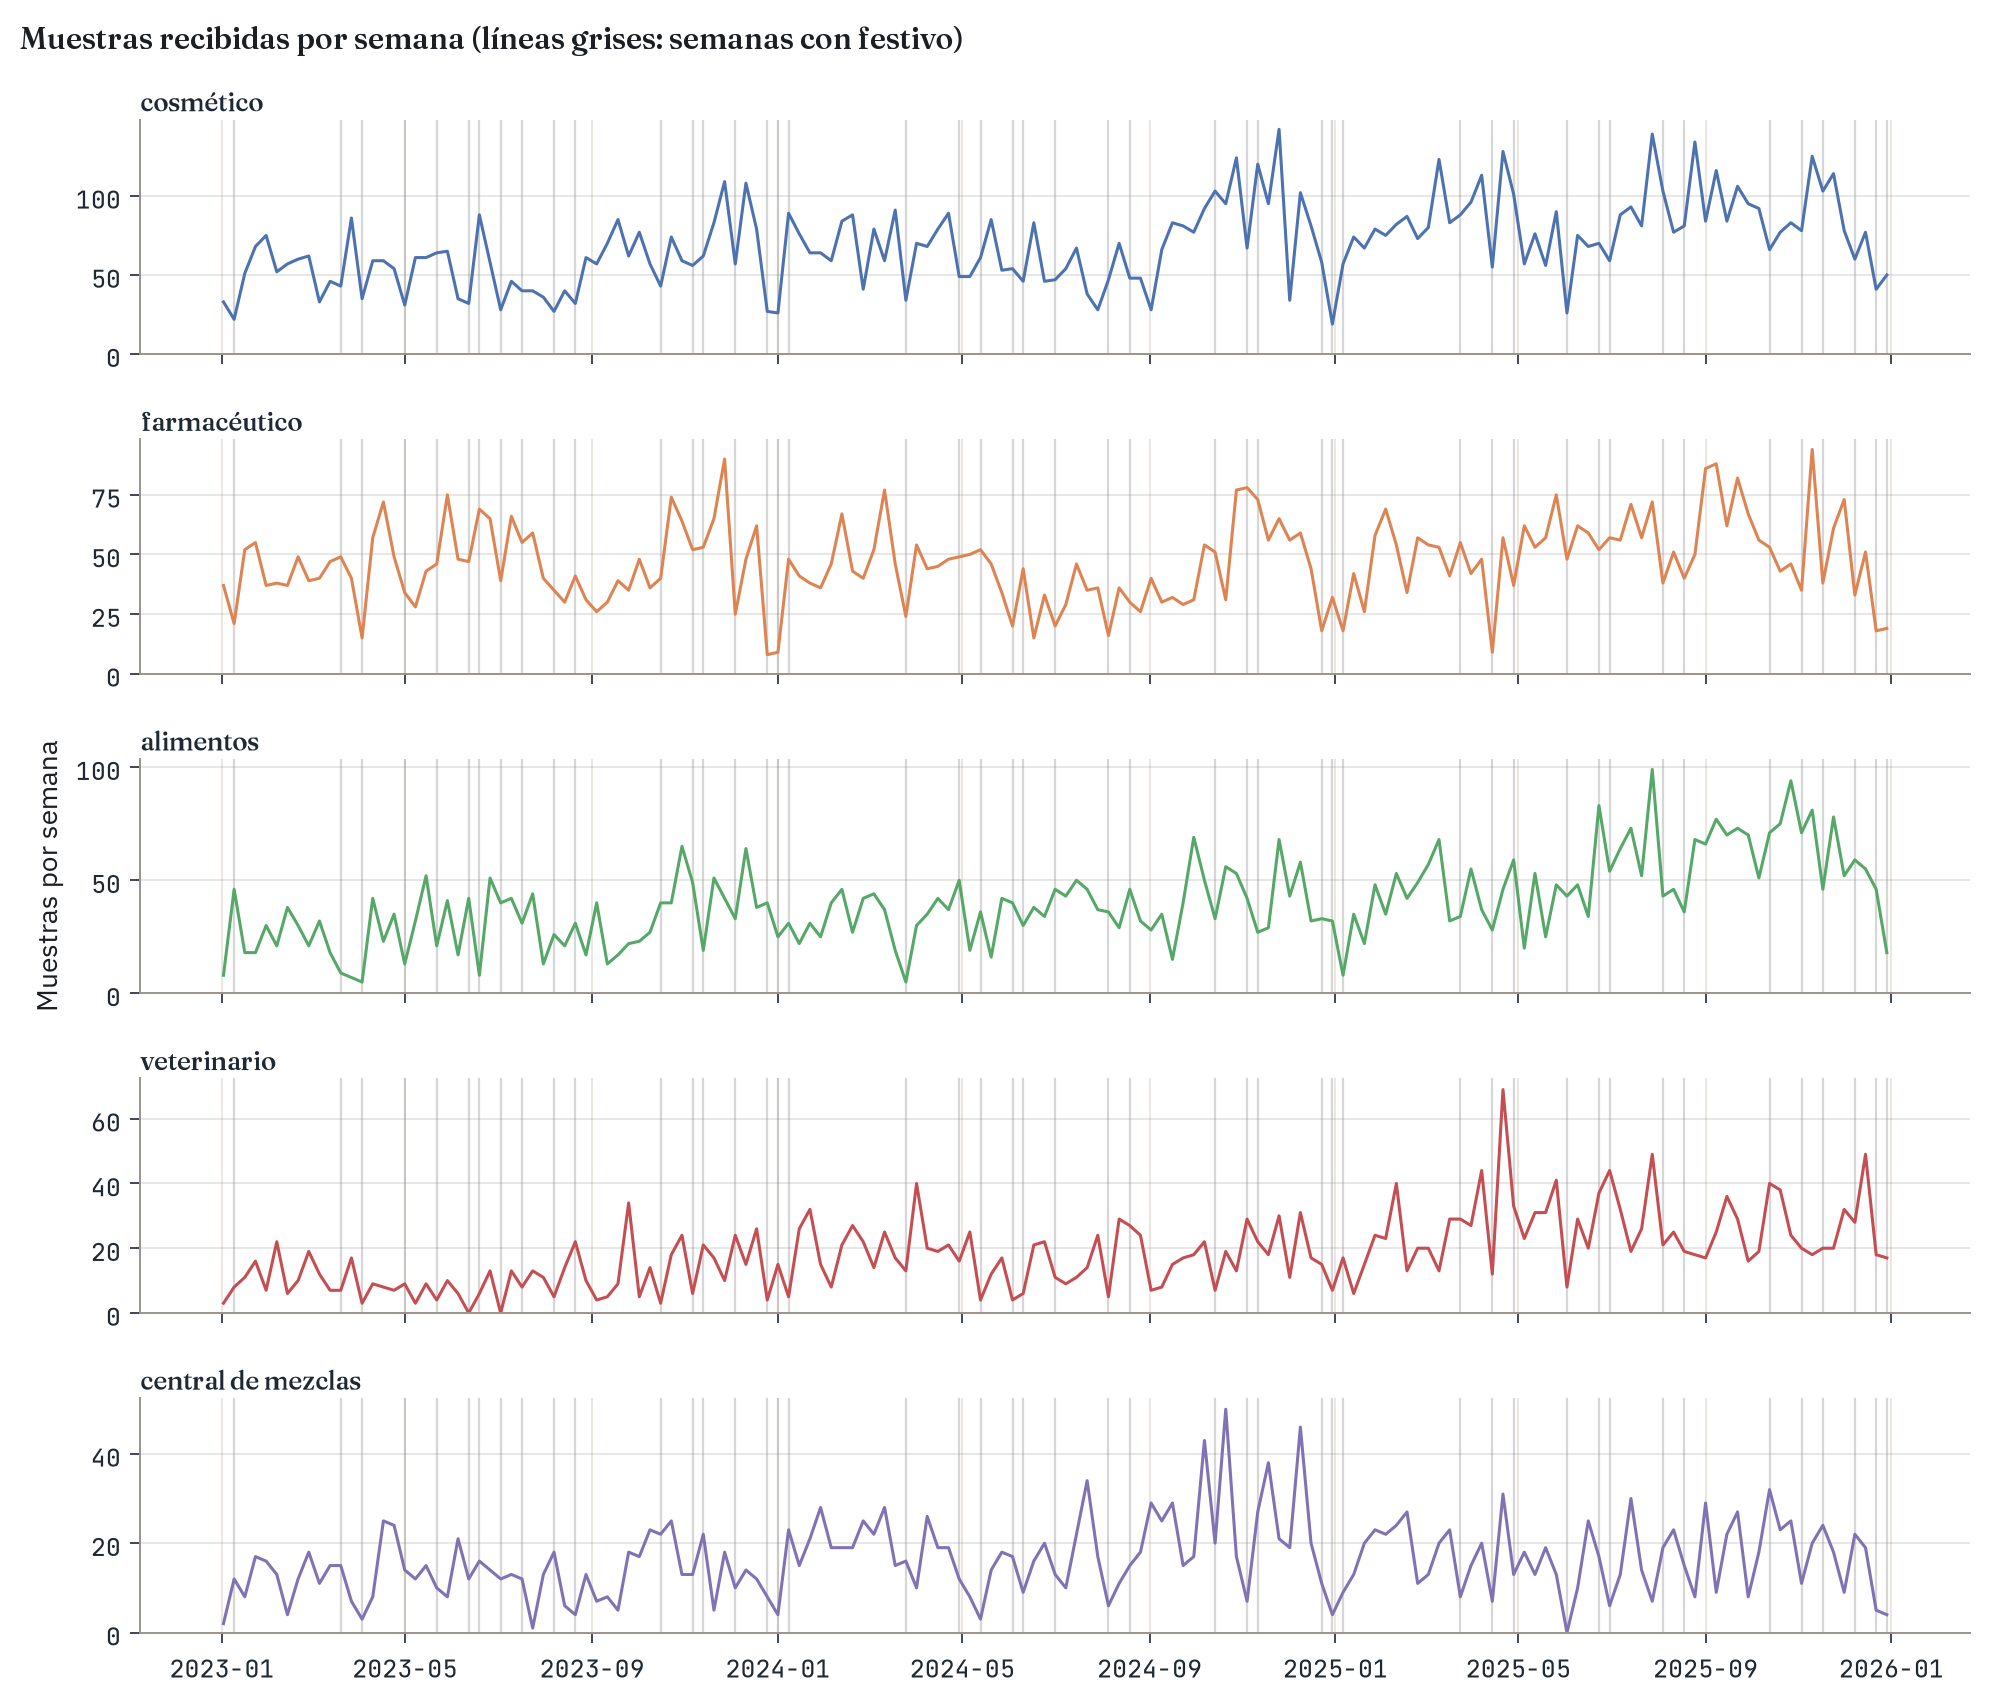
\includegraphics[width=0.7\textwidth]{02_volumen_semanal.png}
\caption{Muestras recibidas por semana en cada línea de negocio durante el
desarrollo. Conviene fijarse en las caídas que coinciden con las semanas con
festivo (líneas grises verticales) y en que las líneas no suben y bajan a la
vez: la carga total depende de la mezcla de clientes de cada día.}
\label{fig:volumen}
\end{figure}

\paragraph{Implicación.} La carga diaria tiene una parte predecible (día de la
semana, festivos, visitas de muestreo programadas y nivel reciente), lo que
justifica un análisis de regresión con variables de calendario y de
programación, siempre con validación temporal, porque la serie no es
estacionaria.

\subsection{No conformidad y sus factores}

Entre las muestras aceptadas del desarrollo, el \ExpTasaNoConformePct{}\,\%
resulta no conforme, es decir, hay unas \ExpConformesPorNoConforme{} conformes
por cada no conforme, y la tasa mensual oscila entre
\ExpTasaMensualMinPct{}\,\% y \ExpTasaMensualMaxPct{}\,\% (con
\ExpTasaPrimerAnioPct{}\,\% en \ExpPrimerAnio{} y \ExpTasaUltimoAnioPct{}\,\%
en \ExpUltimoAnio{}). La Figura~\ref{fig:tasas} muestra que la tasa cambia
según la línea de negocio, la matriz y el ensayo, y la
Figura~\ref{fig:transporte} que las condiciones de transporte importan sobre
todo en combinación: en el cuarto de muestras con transporte más largo la
tasa es de \ExpHorasCuartoAltoPct{}\,\%, frente a \ExpHorasCuartoBajoPct{}\,\%
en el más corto, y algo parecido ocurre con la temperatura
(\ExpTemperaturaCuartoAltoPct{}\,\% frente a \ExpTemperaturaCuartoBajoPct{}\,\%).

\begin{figure}[!htbp]
\centering
\begin{minipage}[t]{0.47\textwidth}\centering
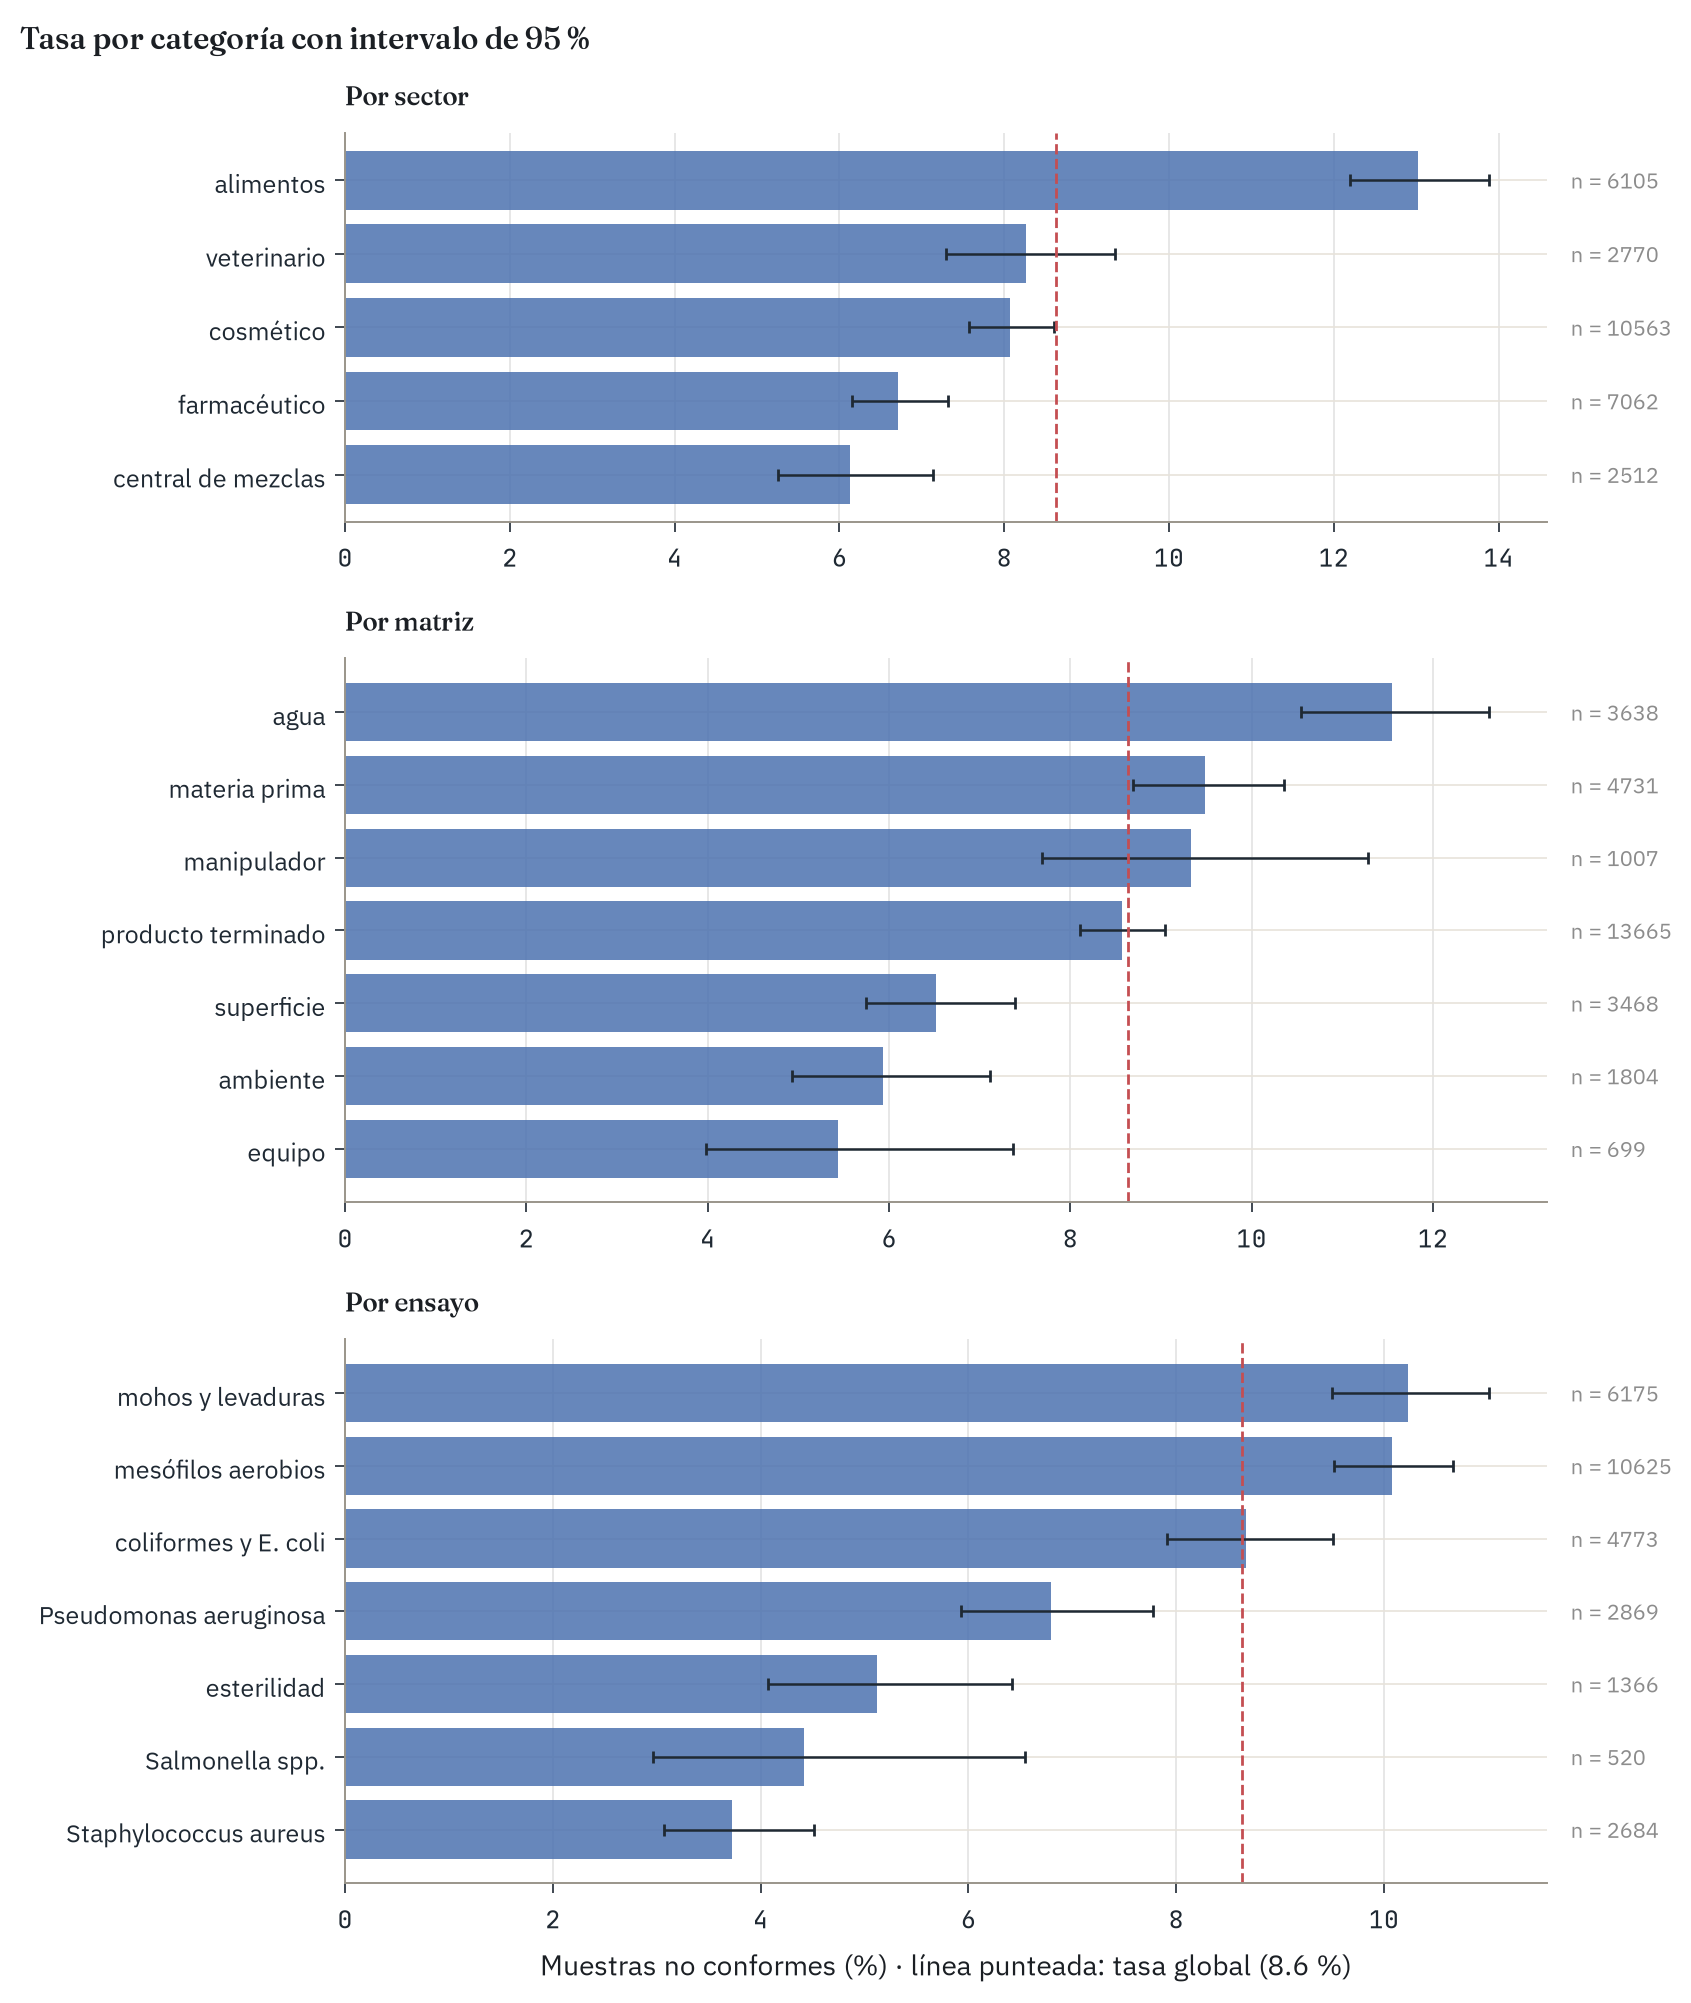
\includegraphics[width=\textwidth]{02_tasa_por_categoria.png}
\caption{Porcentaje de no conformes por línea de negocio, matriz y ensayo,
con intervalo de 95\,\%. La línea punteada es la tasa global; las barras
cuyo intervalo no la cruza son las categorías que de verdad se apartan.}
\label{fig:tasas}
\end{minipage}\hfill
\begin{minipage}[t]{0.49\textwidth}\centering
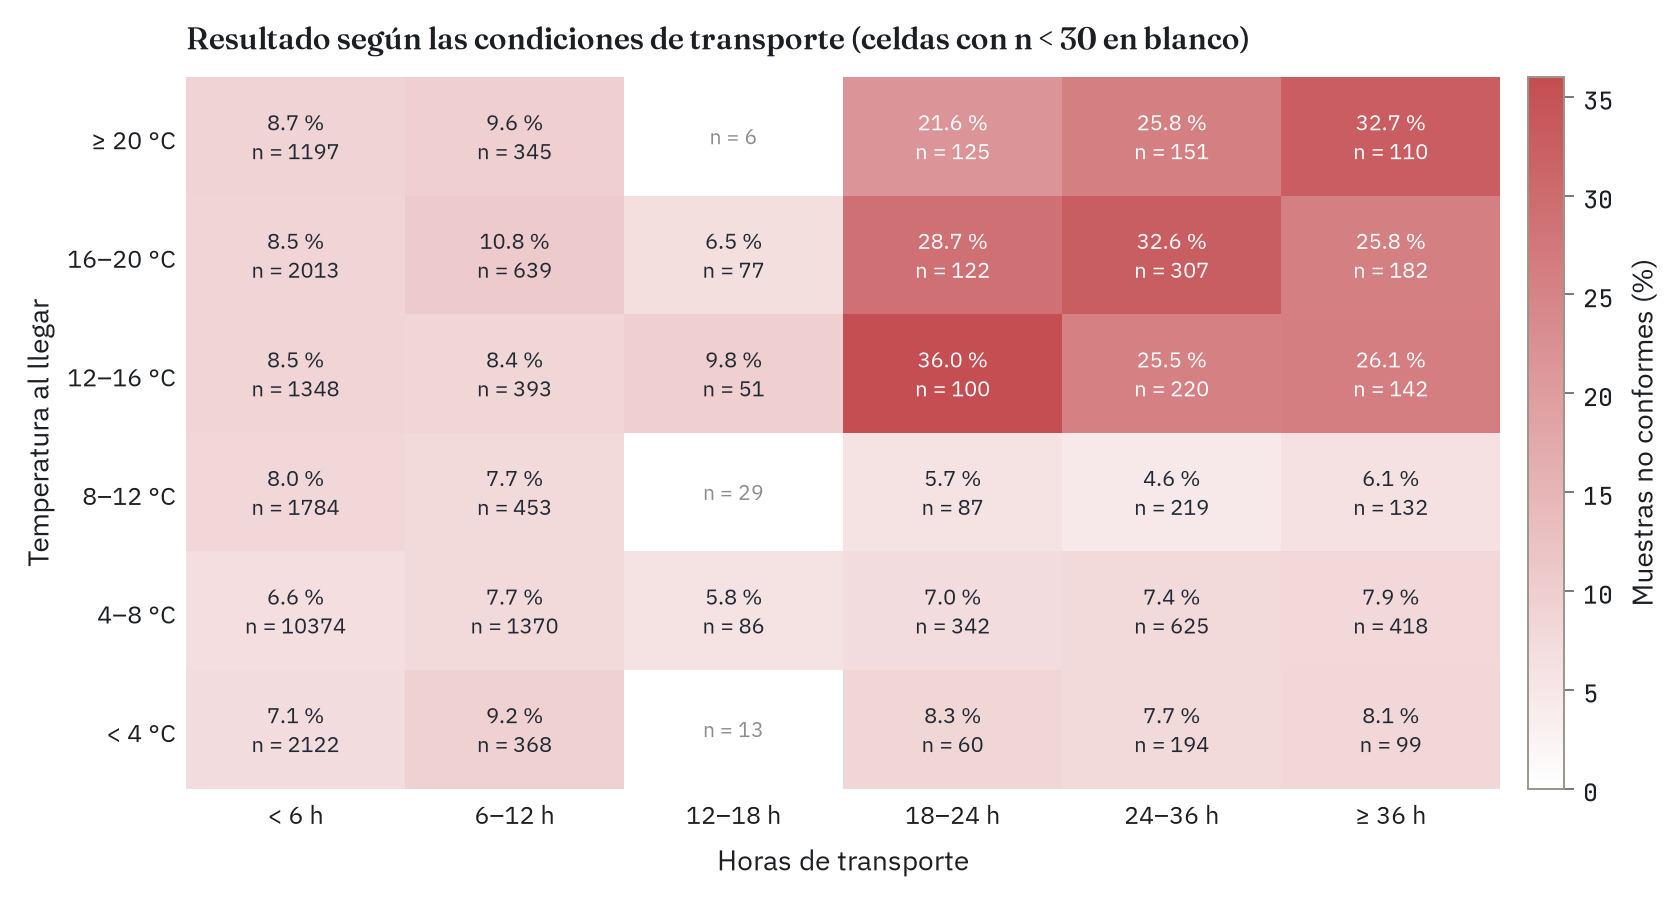
\includegraphics[width=\textwidth]{02_transporte.png}
\caption{Porcentaje de no conformes según horas y temperatura de transporte
(celdas con menos de 30 muestras en blanco). La tasa se dispara en la esquina
superior derecha, donde un transporte largo coincide con una temperatura
alta, y no a lo largo de una sola fila o columna.}
\label{fig:transporte}
\end{minipage}
\end{figure}

Individualmente, ninguna variable explica mucho, ya que la más correlacionada
con la no conformidad, \codigo{\ExpVariableCorrObjetivo}, tiene una
correlación de Spearman de apenas \ExpRhoObjetivo{}, y la variable de llegada
que más separa conformes de no conformes es \codigo{\ExpVariableMasSepara},
con una diferencia de medias de \ExpDiferenciaEstandarMax{} desviaciones
estándar. Entre las variables de entrada, el par más correlacionado
(\codigo{\ExpParCorrelacionado}) tiene $\rho$ de \ExpRhoPar{}, así que no hay
redundancias graves en las variables crudas. Por último, la categórica con
más niveles es \codigo{\ExpCategoriaMasNiveles}, con \ExpNivelesCategoria{}
niveles, y los informes tardan una mediana de \ExpEntregaMediana{} días
(percentil 90 de \ExpEntregaPNoventa{}), con un \ExpEntregaTardiaPct{}\,\%
entregado tarde.

\paragraph{Implicaciones.} Primeramente, el desbalance (una no conforme por
cada \ExpConformesPorNoConforme{} conformes) obliga a medir con ROC-AUC,
precisión media y costo, no con exactitud, y a probar el sobremuestreo como un
factor más. En segundo lugar, la señal es débil y repartida, de forma que se
esperan habilidades moderadas y conviene incluir variables derivadas que
capturen interacciones (como temperatura por horas de transporte) e
historiales recientes por cliente y producto. Finalmente, las categóricas con
muchos niveles exigen agrupar los niveles raros antes de codificar.
